\documentclass[11pt]{article}
\usepackage[margin=0.85in]{geometry}
\usepackage{amsmath,amssymb,booktabs,graphicx,array}
\usepackage[hidelinks]{hyperref}
\usepackage{xurl}
\hypersetup{pdftitle={AFTER: Digital Twins for Cyberattack and Recovery Monitoring in Industrial Robots},pdfauthor={Muhammad Usman}}
\DeclareMathSizes{10}{10}{8}{6}
\setlength{\emergencystretch}{2em}
\setlength{\textfloatsep}{14pt plus 2pt minus 2pt}
\renewcommand{\topfraction}{0.9}
\renewcommand{\textfraction}{0.08}
\renewcommand{\floatpagefraction}{0.8}
\title{AFTER: Digital Twins for Cyberattack and Recovery Monitoring in Industrial Robots}
\author{Muhammad Usman\\[4pt]\small COMSATS University Islamabad, Sahiwal Campus, Pakistan}
\date{}
\begin{document}
\maketitle
\begin{abstract}
A robot can continue to deviate from its intended motion after an unauthorized command ends. A detector that follows recent measurements may lose evidence of that deviation, whereas an inaccurate protected reference may keep an alarm active after recovery. We study this trade-off using a command-driven motion reference, a learned residual correction and explicit alarm-clearance rules. Clean commissioning data select the reference and correction; normal calibration fixes thresholds before attack evaluation. Seventeen controls and ablations are evaluated on 189 synthetic episodes with model mismatch, legitimate command changes and unauthorized motion. The proposed nonlinear correction reduces benign alarm points from 7,156 to 7,012 relative to the uncorrected dual-window reference, but fails the declared improvement criterion: the reduction is 2.01\%, one plant worsens, and pre-return gaps increase. The short window changes no alarm decisions. A following predictor achieves higher schedule F1 but loses evidence before physical return much more often. Separate commissioning, uncertainty and common-input inertial-sensing studies explain limits of reference accuracy and recovery evidence. The results support distinguishing attack detection from physical return and reporting their costs together; they do not establish a novel detector or superiority over published robotic systems.
\end{abstract}
\noindent\textbf{Keywords:} digital twins; industrial robots; anomaly detection; recovery monitoring; system identification; model mismatch.

\section{Introduction}
An industrial robot does not necessarily return to its intended trajectory when an unauthorized command stops. Its position and velocity reflect the earlier disturbance, the controller's response and the plant dynamics. An alarm that clears as soon as prediction error falls can therefore disappear while the robot is still displaced. The opposite error is also possible: the robot returns, but an inaccurate reference keeps the alarm active. These two failures concern the meaning of the reference as much as the accuracy of the detector.

Digital twins provide a useful setting for studying this problem because they connect observations with a representation of the physical process. Recent surveys cover their roles in security monitoring and infrastructure lifecycle security~\cite{securitysurvey,lifecycle}. Those roles require more than a low forecasting error. A reference must represent the behavior relevant to the decision. For an attack alarm, that may be the motion the robot would have followed under approved commands, rather than the next motion most consistent with recent measurements.

Robotic anomaly detectors such as CASPER and its edge-computing successor learn regularities in external motion sensing~\cite{casper,edge}. Hybrid robot twins also combine mechanical, control and learned components~\cite{hybrid}. These approaches motivate prediction-based monitoring, but they do not make all prediction residuals interchangeable. An observation-following predictor may become accurate during a sustained unauthorized trajectory. A command-driven reference can retain the discrepancy, provided its clean initialization and approved-command history remain trustworthy. Its accuracy under legitimate changes then becomes central to false alarms and clearance.

We ask: \emph{when does a command-driven motion reference provide useful evidence for clearing an alarm under model mismatch?} The study assumes a protected copy of approved commands and noisy but honest joint measurements. It tests an explicit candidate: a stable autoregressive reference with a frozen radial-basis correction, followed by short- and long-window return checks. The correction is fitted on clean commissioning data; it cannot learn from an attack during monitoring. This choice makes the information boundary inspectable, but does not establish either algorithmic novelty or physical safety.

The investigation proceeds through five linked validation studies. An initial recovery experiment motivates a clean-data identification study; a separate inertial-sensing study checks predictor training under common inputs; a residual experiment isolates uncertainty in windowed return evidence; and a frozen candidate audit measures detection, false alarms, recovery and component effects together. Later designs use earlier outcomes as development evidence. They do not retroactively become independent confirmations of the earlier hypothesis. This distinction follows the broader need to separate model selection from security evaluation~\cite{arp}.

The contributions supported by the completed work are threefold. First, we specify and test a command-driven reference and alarm-state model with an explicit separation between observed residuals and evaluator-only physical return. Second, matched controls and ablations show that protected reference evolution, nonlinear correction and alarm persistence have different effects: the simpler reference retains the main benefit, while the proposed correction fails its improvement criterion. Third, commissioning and uncertainty diagnostics explain why better prediction alone may not yield usable return evidence. These are empirical and methodological findings. AFTER names the investigation; the present evidence does not validate a new state-of-the-art detector.

\section{Related work}
\subsection{Robot monitoring and reference identification}
CASPER couples external inertial sensing with context-aware industrial-arm anomaly detection~\cite{casper}. The subsequent edge study develops real-time processing for related robotic monitoring~\cite{edge}. Their sensing modality differs from the joint positions, velocities and protected commands used here. We therefore examine independently implemented CNN predictors on a common nominal inertial recording in a separate track. An error measured in that track cannot be interpreted as attack-detection superiority over either complete published system.

Ayankoso et al. combine robot mechanics, drives, control and learned uncertainty accommodation in a hybrid condition-monitoring twin~\cite{hybrid}. Data-driven robot calibration is itself a broad research area~\cite{calibration}; adding a learned correction to a nominal reference is not sufficient evidence of novelty. Classens et al. address structured mechanical-system identification using instrumental variables and block-coordinate descent~\cite{identification}. Our finite autoregressive search uses ordinary least-squares regularization and tests an application-specific recovery requirement, rather than extending that identification theory.

The voraus-AD study provides real robot executions and MVT-Flow, a normalizing-flow anomaly detector~\cite{voraus}. It is a relevant public comparator for an independent real-robot track because both data and author code can be inspected. Its published full-execution likelihood is an offline episode score. Comparing it directly with an online alarm-clearance delay would change the task. FactoryNet extends public industrial data coverage and exposes setpoints, effort, feedback and context in a common schema~\cite{factory}. Its latest manuscript is a preprint, and its releases combine new acquisitions with repackaged sources. Independence must be assessed by acquisition, not by dataset name.

\subsection{Forecasting, uncertainty and runtime decisions}
ModernTCN examines convolutional time-series modeling~\cite{moderntcn}, iTransformer attends across variates for forecasting~\cite{itransformer}, and TimeMixer uses decomposable multiscale mixing~\cite{timemixer}. These recent architectures offer useful forecasting alternatives, but architecture size alone does not solve the reference problem. A more accurate predictor of corrupted motion can be less useful for retaining attack evidence. None of these three systems is claimed as an executed comparator in this study.

Interval-observer fault detection already treats model uncertainty and observer design explicitly~\cite{interval}. FAIL-Detect calibrates uncertainty-aware runtime failure monitors from successful robot rollouts~\cite{fail}. We include a constant episode-band control inspired by that calibration principle in the earlier experiment, without claiming to reproduce its policy-specific signal construction or full method. Howard et al. develop time-uniform confidence sequences~\cite{howard}; our Gaussian window diagnostic uses simpler tail bounds and error spending under stated assumptions.

Kaisar et al. describe a robotic-vehicle cybersecurity architecture involving a kinematic twin, supervisory handover and consistency-gated recovery~\cite{kaisar}. This is close conceptual prior art. The available abstract supports that overlap, but the full algorithm was inaccessible during our audit, leaving an equation-level comparison unresolved. RESCUE uses counterfactual interventions to evaluate the usefulness of runtime alarms~\cite{rescue}. Our counterfactual serves a narrower purpose: measuring when a simulated plant returns to the trajectory it would have followed without command corruption.

Evaluation also matters. TSB-AD examines the reliability of time-series anomaly-detection comparisons~\cite{tsbad}, while VUS studies accuracy measures for temporal anomalies~\cite{vus}. We retain unadjusted point metrics and separately report event detection and recovery. We do not adopt point adjustment or optimize a threshold on test attacks.

\paragraph{Limitations relevant to this comparison.}
The literature supports the individual ingredients of prediction, correction, uncertainty calibration and persistent alarm state. It does not justify treating their combination here as automatically new. The principal comparison gaps are specific: different sensing modalities for CASPER, a full-execution objective for MVT-Flow, unresolved implementation correspondence for some published systems, and missing physical-return labels in public fault data. These are limits on what our experiment can establish, not evidence that the cited systems are generally defective. A claim of superiority requires a compatible implementation and matched information access.

\section{Proposed reference and alarm model}
\subsection{State, information and threat model}
Let $x_t=(q_1,q_2,\dot q_1,\dot q_2)$ be the physical state and $x_t^0$ the state of the same plant under the complete approved command history without corruption. The monitor observes $y_t=x_t+n_t$ and approved position/velocity commands $u_t$. It maintains a history of predicted states and commands, residual buffers, an alarm bit and a return counter. The evaluator alone receives $x_t$, $x_t^0$ and the corruption schedule.

An attacker changes the command delivered downstream of the protected command copy. Commissioning data, the first 100 initialization observations and that copy are trusted. Joint measurements contain noise; this campaign does not test adversarial sensor forgery. Once initialized, the protected reference does not consume new measured states. This prevents those states from changing its parameters or predicted history. It is a conditional information-flow property, not a defense against compromise of both the trusted commands and the sensor channel.

\begin{figure}[t]
\centering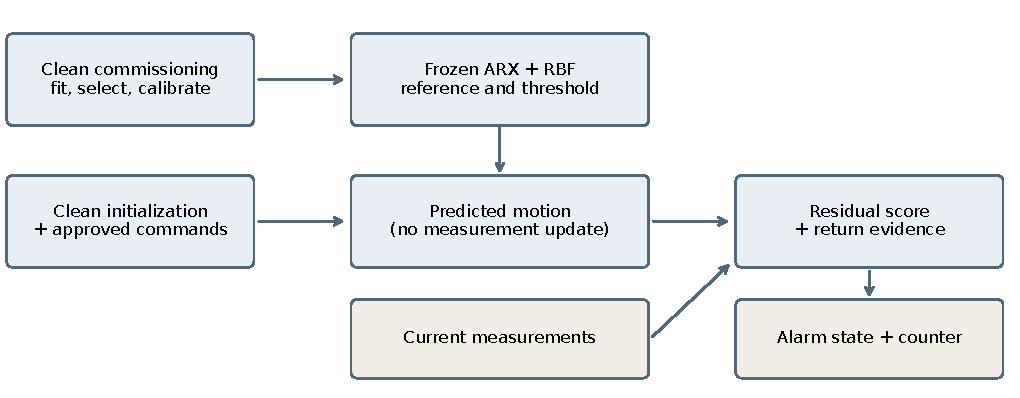
\includegraphics[width=\linewidth]{figures/model.pdf}
\caption{Tested model. Clean data determine the frozen recurrence, correction and threshold. Approved commands drive the reference after initialization. Measurements determine residuals and alarm state; they do not update the reference. Counterfactual physical return is available only to evaluation.}\label{fig:model}
\end{figure}

\subsection{Frozen recurrence and nonlinear correction}
The base is a stable autoregressive model with exogenous inputs (ARX), fitted to clean data. In the fitted coordinate system it has the form
\begin{equation}
 b_t=a+\sum_{k=1}^{p}A_k b_{t-k}+\sum_{k=1}^{p}B_ku_{t-k},
 \qquad r_t^0=\mu+s\odot b_t .\label{eq:base}
\end{equation}
Commands remain in their recorded physical coordinates; $\mu,s$ are training-derived state location and positive scales. The selected orders are 8, 16 and 32 for plants Q1--Q3; the inherited companion matrices have spectral radius below one. After the clean prefix, the recurrence uses its own predictions. These are plant-specific empirical references, not an identified rigid-body twin transferable to an unseen robot.

The correction uses a training-standardized 20-dimensional feature vector,
\[z_t=\operatorname{standardize}_{\rm train}([r_t^0,u_{t-1},u_{t-4},u_{t-16},u_{t-32}]).\] Training-only farthest-point selection supplies centers $c_i$; $h$ is the selected multiplier times the median nonzero distance between centers. With $K$ radial basis functions,
\begin{align}
 \phi_i(z)&=\exp\{-\|z-c_i\|_2^2/(2h^2)\},\\
 r_t&=r_t^0+s\odot W^T[\phi_1(z_t),\ldots,\phi_K(z_t),1]^T .\label{eq:rbf}
\end{align}
The four-output head minimizes $N^{-1}\|\Phi W-E\|_F^2+\lambda\|W_{1:K,:}\|_F^2$, where $E$ contains standardized clean residuals. The intercept is unpenalized. The correction is added to the output, never fed back into the recurrence. Fixed weights and bounded activations bound its magnitude, but do not bound its physical prediction error. A linear correction on the same features tests whether nonlinearity is useful.

\subsection{Alarm entry and return evidence}
Define the standardized residual $e_t=(y_t-r_t)/s$ and score $a_t=\max_j|e_{t,j}|$. A strict exceedance $a_t>\tau$ enters or retains alarm and resets the return counter. Otherwise, the candidate requires
\begin{equation}
 g_t=\mathrm{I}\!\left\{
 \left\|\frac{1}{5}\sum_{k=0}^{4}e_{t-k}\right\|_\infty\le0.1,
 \quad\left\|\frac{1}{41}\sum_{k=0}^{40}e_{t-k}\right\|_\infty\le0.1
 \right\}.\label{eq:gate}
\end{equation}
Ten consecutive eligible points with $g_t=1$ clear an active alarm; entry exceedance has priority. At 50 Hz, the windows contain 0.10 and 0.82 seconds of samples and the dwell contains 0.20 seconds. Signed residual means may cancel oscillatory deviations. Thus the gate tests agreement with the reference, not physical recovery itself. Parameters and thresholds remain fixed throughout each episode, with no reset at attack boundaries.

The physical target is $d_t=\max_j|x_{t,j}-x_{t,j}^0|/s_j$. If reference and noise errors are bounded by $b_t$ and $\eta_t$ in the same norm, the triangle inequality gives $d_t\le a_t+b_t+\eta_t$. A sufficient return condition is therefore $a_t+b_t+\eta_t\le\delta$. It may be impossible when the allowance exceeds $\delta$. Gaussian noise is unbounded, so an empirical maximum is not a deterministic certificate. Supplement S1 gives the conditional bounds and explains why dwell alone cannot repair an infeasible tolerance.

\section{Experiments}
\subsection{Data, simulator and independent evidence}
The attack and recovery results use a horizontal two-joint point-mass arm with coupled inertia, Coriolis terms, damping, saturated proportional--derivative control and optional actuator lag. The plant follows $M(q)\ddot q+C(q,\dot q)+B\dot q=\tau$. Measurements are sampled at 50 Hz; integration uses eight fourth-order Runge--Kutta substeps per sample. Three fixed plant parameterizations vary mass, geometry, damping, lag and sensor noise. Legitimate changes update the approved command; attacks alter only the executed command. Supplement S2 records all physical parameters. Numerical integration checks do not constitute physical validation of an industrial arm.

The separate inertial measurement unit (IMU) study uses the received provider-v2 CASPER nominal file \texttt{IMU\_10Hz.csv}, with nine sensor channels and a recorded SHA-256 identity. Correspondence to the exact original-paper release and timestamp units remains unresolved. We consequently report sample-based prediction error, not physical-time detection delay from its filename. This study contains no attack evaluation.

Before this revision, we independently received the original voraus-AD 100 Hz Parquet file~\cite{voraus} and checked metadata only. It contains 2,122 executions: 1,367 normal and 755 anomalous. The original split contains 948 normal training executions and 1,174 test executions. This is a real acquisition distinct from CASPER; it is not 2,122 independent robots. Process signal values were not inspected, and no model was trained on it. Its fault labels do not establish cyberattacks or physical recovery. FactoryNet remains a source-audited candidate~\cite{factory}; repackaged voraus-AD is not independent evidence. Supplement S6 records permissions, release hashes and comparator-admission issues.

\subsection{Splits, development and calibration}
Simulation fitting uses three clean training episodes per plant. Nine earlier normal episodes select configurations; five separate normal episodes calibrate thresholds. All transformations and RBF centers use training data only. The 30 correction fits comprise eight RBF configurations and two linear configurations for each plant. Selection minimizes worst-episode 99th-percentile residual, then mean root-mean-square error (RMSE), parameter count and identifier. The eight RBF settings cross 32/64 centers, width multipliers 0.5/1 and ridge penalties 0.001/0.01. This is a finite development search, not proof of globally optimal parameters.

Each calibration population has 5,500 eligible scores. The ascending score at rank 5,445 sets the threshold; alarms use strict exceedance. Calibration cannot select models or a different percentile. Equal point-score quantiles do not equalize stateful alarm occupancy or guarantee a future 1\% false-alarm rate. The candidate's normal test uses 81 new task/noise parameterizations. The subsequent attack audit freezes the saved fits, thresholds, 17-method roster and reporting rules before generating 189 episodes.

For the IMU study, raw training rows $[219,9185)$ precede development rows $[9185,12007)$. Splitting precedes the causal 20-sample median filter, scaling and window creation; gaps are rejected. The common eligible populations are 8,192 training targets and 2,048 development targets. Model weights, including CNN checkpoints, are selected on normal development only. Those development errors are not independent final-test estimates. Stochastic fits use seeds 17, 42 and 2026; deterministic controls run once.

\begin{table}[t]
\centering\small
\caption{Five completed validation studies. Their order reflects development; they are not five independent robot datasets. Full protocols and earlier tables are in the supplement.}\label{tab:studies}
\begin{tabular}{>{\raggedright\arraybackslash}p{0.04\linewidth}>{\raggedright\arraybackslash}p{0.22\linewidth}>{\raggedright\arraybackslash}p{0.29\linewidth}>{\raggedright\arraybackslash}p{0.31\linewidth}}\toprule
ID & Question & Evidence & Primary interpretation \\\midrule
E1 & Recovery under mismatch & 216 synthetic episodes; 13 rules & Uncertainty allowance lowers alarms but prevents many clears.\\
E2 & Clean reference accuracy & 63 fits; 81 fresh normal episodes & Better fitting improves allowances; overall feasibility still fails.\\
E3 & Common-input prediction & Nominal CASPER IMU prefix; nine outcomes & AR(4) has lowest development MSE; compact CNN remains training-limited.\\
E4 & Window uncertainty & 36 synthetic residual traces; six rules & Normal-feasibility requirement holds on 20/36 traces.\\
E5 & Candidate and ablations & 30 correction fits; 81 normal and 189 attack-audit episodes & Nonlinear dual-window candidate fails its declared advantage criterion.\\\bottomrule
\end{tabular}
\end{table}

\subsection{Baselines and ablations}
The main audit compares three protected references: base ARX, linear correction and RBF correction. Point rules alarm directly on the thresholded score. Return rules retain alarm until the point, long-window or dual-window evidence meets its criterion, usually for ten samples. A no-dwell ablation isolates persistence. Observation-following references use measured recent history under the same available inputs. Persistence and a causal 21-point rolling mean are simple prediction controls. One-sided cumulative sum (CUSUM) uses a training-only reference statistic and has no alarm reset in this registered implementation. All receive the same episode support; none sees labels or simulator truth.

The IMU track separately compares training mean, persistence, AR(4), a CASPER-style CNN and an Edge-style compact CNN. The latter two are independent implementations with disclosed deviations, not faithful paper-level reproductions. Adamax uses learning rate 0.001, batch size 64, chronological batches and no shuffling; early stopping has patience five and minimum improvement $10^{-6}$, with a 100-epoch cap. MVT-Flow, ModernTCN, iTransformer and TimeMixer have no measured results in this manuscript. Their discussion does not add them to the executed baseline roster.

\subsection{Evaluation measures and success criterion}
The final audit crosses three new tasks, three existing plants, three paired noise seeds and seven conditions: ordinary operation, authorized offset, authorized slowdown, brief offset, persistent offset, hold and slowdown attacks. Each episode contains 1,200 samples with a 100-sample initialization prefix. There are 81 wholly benign and 108 attack episodes, 207,900 eligible points per method, and 25,002 schedule-positive points. Coverage is complete. The continuous scores and alarm arrays are saved before joint label evaluation.

We report unadjusted precision, recall, F1 and average precision (AP), benign alarm points, alarm episodes per eligible benign hour, overlap hits and fresh alarm onsets. A sustained preexisting alarm is an overlap hit but need not be a fresh detection. Physical return is the first start of ten consecutive post-corruption samples with $d_t\le0.1$. This is evaluator-only retrospective labeling. Timely clearing allows 250 samples after that return. Misses remain visible and are excluded only from explicitly conditional clearance denominators.

The registered early-clear count records an alarm falling after first overlap but before stable physical return; it can include a near-onset continuity break while the instantaneous deviation is small. Pre-return gap points measure the associated lost alarm support. An additional, explicitly post-study diagnostic checks deviation at each falling edge. The primary candidate criterion requires no deterioration on the declared plant-level measures and at least a 10\% pooled reduction in benign alarm points or pre-return gaps relative to base dual. Secondary metrics cannot replace this criterion after outcomes are known.

\section{Results}
\subsection{Optimization and clean reference accuracy}
The earlier 63-fit search selected ARX orders 8, 16 and 32 with ridge $10^{-7}$. The new correction search selected 32 RBF centers on every plant, with width multipliers 1, 0.5 and 1 and penalties 0.01, 0.001 and 0.001 for Q1--Q3. Table~\ref{tab:selection} reports the actual selected configurations. ``Selected'' refers to the declared normal-development criterion; it does not mean universally optimal.

\begin{table}[t]\centering\small
\caption{Selected candidate settings and fresh-normal changes relative to the uncorrected reference. A positive error change is worse.}\label{tab:selection}
\begin{tabular}{lrrrrrrr}\toprule
Plant & ARX $p$ & Centers & Width & Ridge & $\tau$ & $\Delta$RMSE (\%) & $\Delta q_{.99}$ (\%) \\\midrule
Q1 & 8 & 32 & 1.0 & 0.01 & 0.036966 & +0.0050 & -0.1314 \\
Q2 & 16 & 32 & 0.5 & 0.001 & 0.037122 & -1.2205 & -1.4022 \\
Q3 & 32 & 32 & 1.0 & 0.001 & 0.057400 & -0.1002 & +0.1506 \\
\bottomrule\end{tabular}

\end{table}

On the 81 fresh normal episodes, the correction changes RMSE by +0.0050\%, $-1.2205$\% and $-0.1002$\% for Q1--Q3. The corresponding 99th-percentile changes are $-0.1314$\%, $-1.4022$\% and +0.1506\%. The all-plant improvement requirement fails. Availability of return evidence on normal data does not establish correct clearing after an attack.

\subsection{Attack detection, false alarms and physical return}
Table~\ref{tab:audit} includes every registered method. RBF dual reduces benign alarm points from 7,156 to 7,012, a 2.0123\% reduction below the required 10\%. Q1 worsens from 2,397 to 2,522. Pre-return gaps rise from two to three, so the non-deterioration condition also fails. Both base and RBF dual overlap all 108 attacks; fresh detections increase from 101 to 105. This secondary gain does not reverse the primary result.

\begin{table}[t]\centering\small\setlength{\tabcolsep}{3pt}
\caption{Complete frozen audit on 189 synthetic episodes. Benign points use 89,100 observations. Hit/fresh means overlap/fresh-onset events; early is the registered continuity-based count; clear is timely clears/detected events with return. AP evaluates continuous entry scores, not retained alarm state.}\label{tab:audit}
\begin{tabular}{lrrrrrrr}\toprule
Method & F1 & AP & Benign & Hit/fresh & Early & Gaps & Clear \\\midrule
base point & 0.7809 & 0.7276 & 853 & 108/108 & 14 & 38 & 108/108 \\
base return & 0.6452 & 0.7276 & 6,811 & 108/101 & 1 & 2 & 108/108 \\
base long & 0.6381 & 0.7276 & 7,156 & 108/101 & 1 & 2 & 108/108 \\
base dual & 0.6381 & 0.7276 & 7,156 & 108/101 & 1 & 2 & 108/108 \\
linear point & 0.7799 & 0.7276 & 895 & 108/108 & 14 & 38 & 108/108 \\
linear dual & 0.6336 & 0.7276 & 7,498 & 108/101 & 1 & 2 & 108/108 \\
RBF point & 0.7816 & 0.7276 & 835 & 108/108 & 14 & 39 & 108/108 \\
RBF return & 0.6482 & 0.7276 & 6,652 & 108/105 & 1 & 3 & 108/108 \\
RBF long & 0.6407 & 0.7276 & 7,012 & 108/105 & 1 & 3 & 108/108 \\
RBF dual & 0.6407 & 0.7276 & 7,012 & 108/105 & 1 & 3 & 108/108 \\
RBF dual, no dwell & 0.7644 & 0.7276 & 1,195 & 108/108 & 1 & 1 & 108/108 \\
following point & 0.9202 & 0.9501 & 867 & 108/108 & 108 & 6,692 & 108/108 \\
following dual & 0.7070 & 0.9501 & 7,635 & 108/105 & 90 & 2,970 & 108/108 \\
RBF following dual & 0.7069 & 0.9501 & 7,678 & 108/105 & 90 & 2,979 & 108/108 \\
persistence & 0.0333 & 0.1016 & 527 & 67/67 & 67 & 15,742 & 67/67 \\
mean (21) & 0.0082 & 0.0867 & 84 & 48/48 & 48 & 11,545 & 48/48 \\
base CUSUM & 0.4198 & 0.1967 & 857 & 108/108 & 0 & 0 & 0/108 \\
\bottomrule\end{tabular}

\end{table}

Following point has F1 0.9202 and AP 0.9501, exceeding RBF dual's 0.6407 and 0.7276, but loses retained evidence before physical return on every attack. Following dual reduces that count to 90, with 2,970 gap points; base dual has one registered early-clear event and two gap points. Figure~\ref{fig:trace} illustrates the distinction. Schedule labels end with command corruption, whereas displaced motion may continue. Retaining an alarm during that interval can improve recovery monitoring and reduce schedule precision simultaneously.

\begin{figure}[t]\centering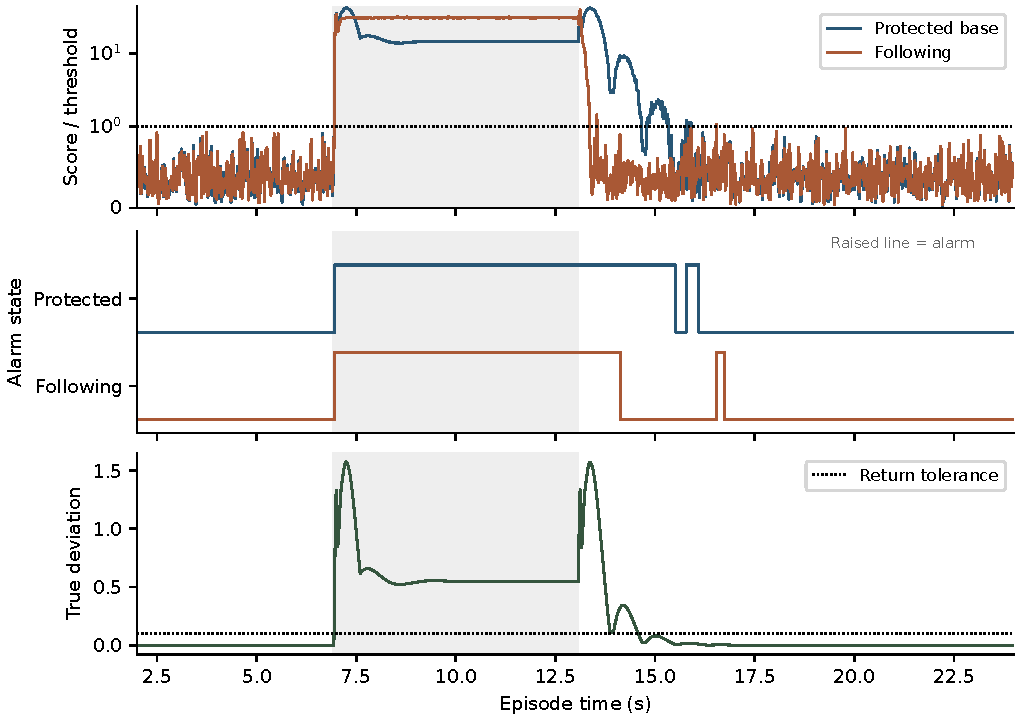
\includegraphics[width=0.94\linewidth]{figures/trace.pdf}
\caption{Post-study illustration from the frozen audit: task N14, plant Q2, seed 17, persistent offset. Shading marks corrupted commands. The following residual falls sooner, although the true deviation remains above the return tolerance. This selected trace illustrates the aggregate comparison; it is not independent confirmation.}\label{fig:trace}
\end{figure}

The single RBF early-clear event occurs two samples after onset while the true standardized deviation is 0.01649, below the 0.1 tolerance. A fresh alarm follows three samples later. It is a continuity break, not evidence of an outside-tolerance clearance. The post-study falling-edge check finds no such outside-tolerance early fall for the protected-reference variants, compared with 108 events for following point and 82 for following dual. This clarification preserves the registered result rather than replacing it. Persistence misses 41 events and the rolling mean misses 60. Their conditional clear ratios therefore cannot be described as complete recovery success.

\subsection{Ablation and diagnostic studies}
Removing the short window changes zero alarm entries across all 189 episodes. Its contribution is unsupported in these conditions. Removing dwell reduces RBF benign alarm points from 7,012 to 1,195 while preserving 108 overlap hits and 108 timely clears. The registered early-clear count remains one, on a different episode. This outcome is informative but cannot be used to promote the no-dwell variant retrospectively as a confirmed new detector. CUSUM retains all detected events with no pre-return gaps but never clears within the declared horizon.

The earlier diagnostics explain why uncertainty handling is difficult. In E1, an empirical allowance reduces benign alarms from 621 to 309 relative to nominal fixed return, but permits timely clearing in only 36/108 detected events with return. With the same entry threshold and no allowance, the comparison rule has 140 benign alarm points and 108 timely clears. E2 reduces the harder plants' allowances by 51.27\% and 38.56\%, yet its overall normal-feasibility requirement fails. E4 meets the declared requirement on only 20/36 synthetic residual traces; temporal correlation and variation within the window limit averaging. These are distinct, versioned experiments, not extra trials from E5.

In E3, AR(4) yields standardized normal-development MSE 0.006074. The three CASPER-style CNN values range from 0.017451 to 0.017703; all stop at 27 epochs and retain epoch 22. The compact CNN values range from 0.042700 to 0.044730 and remain improving at the 100-epoch cap. This is evidence about the inspected implementations and nominal prefix, not a claim that the published neural systems are inferior. Complete results and learning curves are in Supplement S4.

\subsection{Computational cost and verification}
The candidate normal study takes 16.115 seconds wall time and 15.189 seconds worker CPU, with 53.23 MiB sampled peak resident memory. The 189-episode audit takes 27.515 seconds wall and 26.656 seconds worker CPU, with 90.17 MiB sampled peak memory and 83.44 MiB of outputs. These measurements cover shared fitting or evaluation pipelines, not isolated per-method deployment latency. The longer IMU run takes 764.794 seconds wall time, 753.252 seconds CPU and 553.05 MiB sampled memory. The implementation uses local macOS/arm64 environments; Supplement S5 records versions, commands and artifact identities.

The final audit passes 25 synthetic software tests and 30,448 saved-artifact checks, including aligned inference replay and separate metric arithmetic. All 3,213 method--episode outcomes are retained. These checks establish implementation consistency with the declared experiment; they do not provide independent scientific replication. Resource sampling also does not constitute an instantaneous hard memory ceiling.

\section{Discussion and limitations}
The useful distinction is between following measured behavior and retaining a prediction of approved behavior. Protected references preserve evidence in this simulation, but the ordinary ARX already provides that benefit. The nonlinear correction and dual-window assembly do not meet the registered advantage target. Existing identification, residual correction and hysteresis methods remain close prior art. A larger network or a new name would not resolve that missing contribution.

The experiments have limited external validity. Three plant parameterizations share one simplified simulator; seeds repeat stochastic realizations, not independent robot acquisitions. Gravity, contact, flexibility, thermal drift and industrial controller details are absent. Protected command provenance and clean initialization are assumptions, not measured deployment properties. Fault recordings cannot establish adversarial intent, and neither an IMU prediction prefix nor metadata admission provides a real-robot recovery benchmark. No significance test or confidence interval is presented as if the synthetic episodes were independent industrial trials.

The new voraus-AD acquisition supports a concrete next comparison with MVT-Flow in a separate offline track. Its manuscript-to-code discrepancies must be resolved or disclosed, and a split contract must be frozen before observation development. FactoryNet offers additional acquisition leads, but source overlap, context-label leakage and release completeness require care. The outcome-informed redesign of the current candidate is exploratory. A new confirmatory claim needs compatible baselines and fresh evidence that were not used to choose the replacement.

\section{Conclusion}
Attack detection and physical recovery require different evidence. A protected command-driven reference retains deviations that a following predictor can absorb, but model error and alarm persistence create substantial false-alarm costs. The tested nonlinear dual-window candidate fails its declared improvement criterion, and its short window changes no decisions. These results support evaluating reference accuracy, detection and clearance together. They do not establish a novel detector or superiority over CASPER; compatible published-method reproduction and independent recordings remain necessary.

\section*{Declarations}
\paragraph{Funding and competing interests.} No funding or competing interests were declared.
\paragraph{Data and code.} Versioned code, configurations, result artifacts and a reproducibility inventory are retained locally. No public repository release is claimed. Third-party data remain subject to their providers' terms; the supplement records source identifiers and hashes.
\paragraph{AI assistance.} OpenAI Codex assisted with literature searches, code, experiment execution, analysis, writing and editing. The named author must review the scientific claims and approve the manuscript before submission. No independent human review or completed author-contribution attestation is asserted here.
\begingroup\small
\begin{thebibliography}{20}

\bibitem{securitysurvey} Abdul Rehman Qureshi, Adrián Asensio, Muhammad Imran, Jordi Garcia, Xavi Masip-Bruin. {A survey on security enhancing Digital Twins: Models, applications and tools}. \emph{Computer Communications, 238:108158}, 2025. Article 108158. \url{https://doi.org/10.1016/j.comcom.2025.108158}.

\bibitem{lifecycle} Taru Itäpelto, Mohammed Elhajj, Marten van Sinderen. {Digital twin application in lifecycle security of critical infrastructures: A systematic literature review}. \emph{International Journal of Critical Infrastructure Protection, 50:100783}, 2025. Article 100783. \url{https://doi.org/10.1016/j.ijcip.2025.100783}.

\bibitem{casper} Hakan Kayan, Ryan Heartfield, Omer Rana, Pete Burnap, Charith Perera. {CASPER: Context-Aware IoT Anomaly Detection System for Industrial Robotic Arms}. \emph{ACM Transactions on Internet of Things, 5(3):1--36}, 2024. Article 18. \url{https://doi.org/10.1145/3670414}.

\bibitem{edge} Hakan Kayan, Ryan Heartfield, Omer Rana, Pete Burnap, Charith Perera. {Real-Time Anomaly Detection for Industrial Robotic Arms Using Edge Computing}. \emph{IEEE Internet of Things Journal, 12(15):29696--29712}, 2025. \url{https://doi.org/10.1109/JIOT.2025.3569780}.

\bibitem{hybrid} Samuel Ayankoso, Eric Kaigom, Hassna Louadah, Hamidreza Faham, Fengshou Gu, Andrew Ball. {A Hybrid Digital Twin Scheme for the Condition Monitoring of Industrial Collaborative Robots}. \emph{Procedia Computer Science, 232:1099--1108}, 2024. \url{https://doi.org/10.1016/j.procs.2024.01.108}.

\bibitem{arp} Daniel Arp, Erwin Quiring, Feargus Pendlebury, et al.. {Pitfalls in Machine Learning for Computer Security}. \emph{Communications of the ACM, 67(11):104--112}, 2024. \url{https://doi.org/10.1145/3643456}.

\bibitem{calibration} Tinghui Chen, Weiyi Yang, Shuai Li, Xin Luo. {Data-Driven Calibration of Industrial Robots: A Comprehensive Survey}. \emph{IEEE/CAA Journal of Automatica Sinica, 12(8):1544--1567}, 2025. \url{https://doi.org/10.1109/jas.2025.125237}.

\bibitem{identification} Koen Classens, Rodrigo A. Gonz{\'a}lez, Tom Oomen. {Recursive identification of structured systems: An instrumental-variable approach applied to mechanical systems}. \emph{European Journal of Control, 84:101238}, 2025. \url{https://doi.org/10.1016/j.ejcon.2025.101238}.

\bibitem{voraus} Jan Thieß Brockmann, Marco Rudolph, Bodo Rosenhahn, Bastian Wandt. {The voraus-AD Dataset for Anomaly Detection in Robot Applications}. \emph{IEEE Transactions on Robotics, 40:438--451}, 2024. \url{https://doi.org/10.1109/tro.2023.3332224}.

\bibitem{factory} Jonas Petersen, Pratik Jawahar, Riccardo Maggioni, et al.. {FactoryNet: A Large-Scale Dataset toward Industrial Time-Series Foundation Models}. \emph{arXiv preprint}, 2026. Preprint, version 5, 8 October 2026; arXiv:2605.09081. \url{https://arxiv.org/abs/2605.09081v5}.

\bibitem{moderntcn} Donghao Luo, Xue Wang. {ModernTCN: A Modern Pure Convolution Structure for General Time Series Analysis}. \emph{International Conference on Learning Representations}, 2024. \url{https://openreview.net/forum?id=vpJMJerXHU}.

\bibitem{itransformer} Yong Liu, Tengge Hu, Haoran Zhang, et al.. {iTransformer: Inverted Transformers Are Effective for Time Series Forecasting}. \emph{International Conference on Learning Representations}, 2024. \url{https://openreview.net/forum?id=JePfAI8fah}.

\bibitem{timemixer} Shiyu Wang, Haixu Wu, Xiaoming Shi, et al.. {TimeMixer: Decomposable Multiscale Mixing for Time Series Forecasting}. \emph{International Conference on Learning Representations}, 2024. \url{https://openreview.net/forum?id=7oLshfEIC2}.

\bibitem{interval} Jordi Meseguer, Vicen{\c c} Puig, Teresa Escobet, Jordi Saludes. {Observer gain effect in linear interval observer-based fault detection}. \emph{Journal of Process Control, 20(8):944--956}, 2010. \url{https://doi.org/10.1016/j.jprocont.2010.06.017}.

\bibitem{fail} Chen Xu, Tony Khuong Nguyen, Emma Dixon, et al.. {Can We Detect Failures Without Failure Data? Uncertainty-Aware Runtime Failure Detection for Imitation Learning Policies}. \emph{Robotics: Science and Systems XXI}, 2025. \url{https://doi.org/10.15607/RSS.2025.XXI.073}.

\bibitem{howard} Steven R. Howard, Aaditya Ramdas, Jon McAuliffe, Jasjeet Sekhon. {Time-uniform, nonparametric, nonasymptotic confidence sequences}. \emph{The Annals of Statistics, 49(2):1055--1080}, 2021. \url{https://doi.org/10.1214/20-AOS1991}.

\bibitem{kaisar} H. Kaisar, M. Rehan, I. Ahmed, M. Bilal, M. Khalid. {A Digital Twin-Based Cybersecurity Architecture for FDI Anomaly Detection and Isolation in Next Generation Robotic Vehicles}. \emph{IEEE Open Journal of the Communications Society, 7:12709--12728}, 2026. \url{https://doi.org/10.1109/OJCOMS.2026.3739185}.

\bibitem{rescue} David Ahmedt-Aristizabal, Abdelwahed Khamis, Mohammad Ali Armin, Lars Petersson. {RESCUE: Is This Alarm Worth Acting On? Counterfactual Evaluation of VLA Runtime Monitors}. \emph{arXiv preprint}, 2026. Preprint, version 1, 9 October 2026; arXiv:2610.13516. \url{https://arxiv.org/abs/2610.13516v1}.

\bibitem{tsbad} Qinghua Liu, John Paparrizos. {The Elephant in the Room: Towards A Reliable Time-Series Anomaly Detection Benchmark}. \emph{Advances in Neural Information Processing Systems 37, 108231--108261}, 2024. \url{https://doi.org/10.52202/079017-3437}.

\bibitem{vus} Paul Boniol, Ashwin K. Krishna, Marine Bruel, et al.. {VUS: effective and efficient accuracy measures for time-series anomaly detection}. \emph{The VLDB Journal, 34(3)}, 2025. Article 32. \url{https://doi.org/10.1007/s00778-025-00907-x}.

\end{thebibliography}

\endgroup
\end{document}
